\documentclass[superscriptaddress,twocolumn,pre]{revtex4}
\bibliographystyle{apsrev}

\usepackage{ifthen}
\newboolean{pnas}
\setboolean{pnas}{false}

\usepackage{amsmath}
\usepackage{amsfonts}
\usepackage{amssymb}
\usepackage{mathtools}
\usepackage{graphicx}
\usepackage[T1]{fontenc}
\usepackage[utf8]{inputenc}
\graphicspath{{images/}}
\usepackage{color}
\usepackage[pdfstartview=FitH,
            breaklinks=true,
            bookmarksopen=false,
            bookmarksnumbered=true,
            colorlinks=true,
            linkcolor=black,
            citecolor=black,
            urlcolor=black,
            pdftitle={Peptidome},
            pdfauthor={Andreas Mayer},
            pdfsubject={}
            ]{hyperref}
\newcommand{\B}{\boldsymbol}
\newcommand{\ud}{\mathrm{d}}
\newcommand{\<}{\langle}
\renewcommand{\>}{\rangle}

\def\(({\left(}
\def\)){\right)}                       
\def\[[{\left[}
\def\]]{\right]}

\newcommand{\AM}[1]{{\color{blue}#1}}

\begin{document}

\title{A statistical ensemble approach to immune discrimination}
%\author{Andreas Mayer}
%\author{Quentin Marcou}
%\author{Marta Luksza}
%\author{Ben D Greenbaum}
%\author{William Bialek}
\date{\today}

\begin{abstract}
The immune system needs to distinguish molecular signatures of pathogens from those found in the organisms' own proteins. A naive, but universal way to discriminate is to whitelist everything that should not elicit a reaction. Can the immune system do better? To begin to answer this question we characterize the self and pathogen proteomes as statistical ensembles. Probabilistic models reveal how both universal and phyla-specific constraints on protein evolution shape the statistics of the proteomes. The models furthermore allow us to quantify to what extent the ensembles differ systematically. We analyze whether and how these differences might be used for efficient immune defense. Finally, we compare predictions to what is known about epitopes recognized by the immune system. 
\end{abstract}

\maketitle

\section{Ideas}


Are there any features that distinguish foreign antigens from self-antigens? There is one view of adaptive immunity in which both self and non-self antigens are random samples from a common (and essentially flat) distribution of peptides of a given length. Discrimination is then achieved solely on the basis of "white-listing": thymic negative selection acts to get rid of those cells that are reactive to self, leaving everything else as potentially foreign. If the two types of antigens are instead drawn from different distributions, than some regions of antigenic space will be much more likely to be self and some much more likely to be non-self. Over evolutionary timescales the recombination machinery might then have evolved to bias the immune repertoire towards recognizing antigens that are more unlikely to arise from the human proteome.

If such differences exist they may arise from species-dependent codon biases or differences in the GC content of the DNA. Additionally due to different types of proteins and different types of environments the amino acids needed for proper functioning of a protein might differ between a host and its pathogen. On the other hand, however, coevolution of the pathogens might select that they have a more similar distribution than they would otherwise have. One way to test for this is whether pathogens adapted to a particular host are particularly similar to its peptidome.

Maybe the immunogenicity of an antigen is related to how untypical it is given the normal distribution of the human proteome. One could try and check this by looking at known antigens from the immuno-epitope database (IEDB). Are they less typical of the human ensemble? This could be a useful insight for cancer immunotherapy: Are good neoantigens those that represent large perturbations from the normal distribution towards the pathogen distribution? Interestingly, for neoantigen prediction Luksza et al. \cite{Luksza2017} have found that how well a neoantigen aligns to known viral/bacterial antigens is a predictor of its immunogenicity. The same idea could also be of relevance for autoimmunity, where more uncommon peptides within the self-peptidome might also be more likely to lead to autoimmunity.

It could be interesting to also consider abundance information (see e.g. \url{https://pax-db.org/}), i.e. weigh a peptide by the abundance of the protein from which it arises. In cancer immunology \cite{Walz2015} it has been argued that immune activation can be achieved not just by neoantigens but also by large changes in protein abundance. One might hypothesize that peripheral tolerance mechanisms can get overwhelmed by large amounts of an otherwise untypical antigen.

Another interesting connection to make would be to whether mitochondrial (or mitochondria-associated) proteins show a more similar distribution to foreign antigens than others. Due to their evolutionary relationship to bacteria they might show a different distribution. The immune system might use mitochondrial antigens to bias the repertoire towards the relevant regions by positive selection.

There is quite a lot of data in a single proteome. Consider e.g. homo sapiens: 20000 genes times 1000 amino acids per gene on average gives $2 \cdot 10^7$ possible peptides, when not accounting restrictions on what can be presented on MHCs (number of peptides $\approx$ length, as you can start a peptide in any position). This also implies that most 5mers will still be represented in the proteome, as there are only $20^5 = 3.2 \cdot 10^6$ possible 5mers.

Small changes in amino acid usage can lead to larger changes in the relative likelihood of longer stretches of otherwise random sequences: consider a 10\% difference for single amino acids than a random 8mer has a loglikelihood ratio of $1.1^8 \approx 2.15$. Even larger likelihood ratios are expected for long kmers once pairwise or higher-order correlations are considered (see \cite{Schneidman2006} for an example of this).

In terms of modeling we could build a maximum entropy distribution constrained to reproduce the amino acid frequencies and the correlations between pairs of amino acids a given distance apart (as we consider random substrings the distribution should only depend on absolute distance). This is quite reminiscent of what was done by Mora et al. \cite{Mora2010} for the distribution of antibodies.

There is also other type of efforts that we could link to: There is the emerging field of immunopeptidomics, and we could also try and build models for HLA-restricted amino acid distributions.
On a more general level the question which structural constraints restrain the evolution of amino acid patterns has received attention for a long time \cite{Turjanski2018}. Random strings of amino acids do not yield valid, folding proteins, but amino acid strings of natural proteins are hard to distinguish from random.


\section{Prior work}

Karlin and Bucher \cite{Karlin1992} have shown the existence of pairwise correlations in amino acid usage and discuss various structural reasons for these correlations. Peer et al. \cite{Peer2004} have shown that amino acid and oligopeptide compositions differentiate among phyla, which is a very encouraging finding for the premise of this project. There has also been follow up work with similar conclusions \cite{Bogatyreva2006}. On the other hand \cite{Lavelle2009} claims that generally 4mers and 5mers do not show large deviations from random models when taking care to remove bias by large protein families.

Another interesting line of work has involved low-complexity sequences within proteins (see \cite{Cascarina2018} and references therein).

There has been some early work about peptide similarity in the context of immunology by Burroughs, De Boer, and Kesmir \cite{Burroughs2004}. Interestingly, they demonstrate that the number of shared 9mers decreases with evolutionary distance, and is much lower for e.g. human and bacteria than for human and mouse, or human and drosophila. The paper also discusses some possible slight preference of the antigen processing pathway for non-self antigens. In a follow up work an overlapping set of authors build a tool for immunogenicity prediction based on small differences in amino acid usage in recognized epitopes \cite{Calis2013}. A more recent follow up by Wortel et al. \cite{Wortel2018} shows that self and foreign peptides are largely similar (much more similar then words from different languages). They then argue that under these conditions thymic selection should minimizie the co-occurrence of similar self-peptides for efficient self/non-self discrimination based on negative selection. 

Coevolution \cite{Bahir2009}.

Under the heading of immunopeptidomics and MHC ligandomics efforts are underway to use mass-spectrometry to identify peptides that might be seen by the adaptive immune system \cite{Abelin2017,Liepe2016}. Two of the labs contributing to this effort are those of S Stefanovic (U Tuebingen) and Ruedi Aebersold (ETH Zuerich).

\section{Results}

\subsection{Proteins are surprisingly random}

\begin{figure}
    \includegraphics{entropykmer}
    \caption{Entropy of the kmer distribution of the human and yeast proteome. The solid black line shows the maximal entropy of the flat distribution over the 20 possible amino acids $\log_2 20$. Note how the biggest reduction in entropy comes from amino acid biases with only a small further reduction by correlations in amino acid usage.
    \label{figentropykmer}
    }
\end{figure}


\begin{figure}
    \includegraphics[width=\columnwidth]{mutualinformationdecay}
    \caption{Mutual information between amino acids a certain distance apart in the human and mouse proteome. The mutual information is small as compared to the entropy of the single site $\sim 4$ bits, but extends to long distances. The prominent peaks at a distance that is a multiple of 28 amino acids in the human proteome are likely due to Zinc-finger repeats, more particularly C2H2 fingers (cf. high fold enrichments of cysteine and histdine at a distance of 28) \cite{Krishna2003}. 
    \label{figmutualinformationdecay}
    }
\end{figure}

How close to random is the protein distribution? To answer this question we calculate how much information about the amino acid in a certain position is revealed by knowing its neighbors. Concretely, we calculate the mutual information between amino acid pair a certain distance apart. The mutual information can be expressed as $I(X, Y) = H(X) + H(Y) - H(X, Y)$. We use this expression to calulate the mutual information from the single site entropies and the entropy of the joint distribution, which we calculate using the estimator proposed by Grassberger \cite{Grassberger2003}. (TODO: Use NSB estimator instead?) Note that one cannot assume uniform single site entropies across all comparions stemming most notably from differences in amino acid composition for the first few amino acids within a protein (Fig.~\ref{figentropyaa}). The universal constraints on unrelated proteins are surprisingly small as measured by the mutual information (Fig.~\ref{figmutualinformationdecay}, see also \cite{Lavelle2009}). 


We can further dissect which correlations between individual amino acids contribute to the mutual information. To do so we analyze the fold enrichment of amino acid doublets relative to an independent model. Most doublets are only over- or underrepresented moderately (Fig.~\ref{figdoubletentrichment}). An exception is a strong enrichment of Cysteine-Cysteine 3 amino acids apart. This enrichment has been found previously \cite{Greenbaum2014} and is likely due to a particular preference of cysteines to form disulfide bonds at this distance. Another prominent feature of this data are the relatively high enrichments along the diagonal at all distances. This might be attributable to amino acid repeats within some proteins \cite{Turjanski2018}.

\begin{figure}
    \includegraphics[width=\columnwidth]{doubletenrichment}
    \caption{Doublets are only enriched moderately relative to independent amino acid choice. (The enrichments are statistically significant, however. There are $\sim 10^7$ amino acids in the human proteome and thus on the order of $\sim 10^4$ counts per doublet. The relative error on the frequencies is thus on the order of only $\sim 1/\sqrt{10^4} = 10^{-2}$.)
    \label{figdoubletentrichment}
    }
\end{figure}

\subsection{The distribution of kmer likelihoods is close to being lognormal}

\begin{figure}
    \includegraphics{lognormalaa}
    \caption{Histogram of amino acid frequencies in the human proteome and lognormal approximation. (A) Probability density of the empirical likelihoods of a randomly drawn single amino acid and lognormal approximation. (B) Probability density of the empirical likelihoods of a randomly drawn 4-mer and lognormal prediction based on an independent model.
    (C) Probability density of the likelihoods of randomly drawn 9-mers under an independent model and lognormal prediction.
    \label{figlognormalaa}
    }
\end{figure}

As the two-point correlations are small we can try and approximate the likelihood of a given kmer in a proteome by an independent site model,
\begin{equation}
    P(s_1s_2 ... s_k) = \prod_{i=1}^k P(s_i),
\end{equation}
or more conveniently, their log-likelihood
\begin{equation}
    \ln P(s_1s_2 ... s_k) = \sum_{i=1}^k \ln P(s_i),
\end{equation}
which is a sum of independent random variables under the independent site model.
Using the central limit theorem we can approximate the distribution of the log-likelihoods of a kmer by a normal distribution. To do so we need to know the mean $\mu$ and variance $\sigma^2$ of the likelihood of a randomly picked amino acid. These can be calculated directly from the probability mass function of amino acid frequencies (Fig.~\ref{figlognormalaa}A). Note that the distribution of amino acid frequencies is somewhat skewed (skewness $\gamma_1 = -1.05$), but this skewness should diminish with $k$. The kmer distribution is approximately normal with mean $k \mu$ and variance $k \sigma^2$ as the cumulants of the sum of independent variables is equal to the sum of the cumulants.  Indeed, using the mean and variance of the distribution of frequencies of randomly chosen amino acids (Fig.~\ref{figlognormalaa}A), predicts relatively well the mean and variance of the empirical likelihoods of 4mers (Fig.~\ref{figlognormalaa}B) as well as of the model-based likelihoods of 9mers (Fig.~\ref{figlognormalaa}C). There are some deviations from the lognormal approximation apparent in both cases. There is a slight shift towards higher mean likelihoods, corresponding to a slightly reduced entropy in line with our earlier findings. Additionally, there are enrichments at the lower tail in both distributions, and the 4mer data shows an additional enrichment at the high likelihood tail.


\subsection{Quantifying differences between human and pathogen proteomes}

As argued above the dominant statistical bias away from a uniform peptide distribution arises from single amino acid biases. Therefore to start unraveling potential differences between human and pathogen proteomes we can quantify how much the distributions of single amino acids differs between proteomes. The overall differences can be quantified using the Kullback-Leibler divergence between the distribution of amino acid usage in a pathogen proteome and the human proteome. It turns out that these differences are small with some notable exceptions (Table~\ref{tabkldiv}). Interestingly, the parasite Plasmodium falciparum has the largest observed divergence from the human amino acid usage, which might be a result of the known AT bias of its genome \cite{Hamilton2017}. Vaccinia is higher than other viruses, which might attributable to it replicating outside the nucleus of the host cell using its own set of proteins for DNA replication and gene transcription \cite{Tolonen2001}. Mostly the Kullback-Leibler divergences between the doublet distributions are about twice the single site divergences. Notable exceptions are some of the viral proteomes, but this might be due to finite sampling effects biasing the entropy estimates for these small proteomes.

The Kullback-Leibler divergence is exactly the expected log-likelihood ratio drawing an amino acid from the pathogen distribution versus the human distribution. Under the independent model log-likelihoods are additive and thus the average log-likelihood ratio for a kmer is simply k times the calculated single site $D_{KL}$.
%In the limit of large $k$ 
%Chernoff-Stein Lemma!

\begin{table}
    \begin{center}
        \begin{tabular}{ c c c }
            Organism&site $D_{KL}$&doublet $D_{KL}$\\
            \hline
Mouse&0.00023&0.00089\\
Yeast&0.046&0.097\\
Cockroach&0.015&0.033\\
Cattle&0.00031&0.0011\\
Chicken&0.0011&0.0038\\
Wheat&0.012&0.029\\
Soybean&0.013&0.033\\\hline
Vaccinia&0.13&0.27\\
InfluenzaB&0.043&0.17\\
InfluenzaA&0.042&0.17\\
CMV&0.035&0.085\\
HCV&0.064&0.2\\
HBV&0.078&0.28\\
DENV&0.049&0.19\\
HIV&0.043&0.19\\
EBV&0.043&0.1\\ \hline
Human viruses&0.015&0.038\\\hline
Ebola&0.023&0.12\\
Tuberculosis&0.11&0.23\\
Listeria&0.071&0.15\\
Burkholderia&0.1&0.23\\
Meningococcus&0.039&0.1\\
StreptococcusPyogenes&0.06&0.14\\
Hpylori&0.077&0.19\\
Lyme&0.19&0.38\\
Tetanus&0.15&0.3\\ 
Leprosy&0.077&0.17\\ \hline
Malaria&0.36&0.71\\
Chagas&0.017&0.051\\
OnchocercaVolvulus&0.03&0.069\\
        \end{tabular}
    \end{center}
    \caption{Kullback-Leibler divergence between amino acid frequencies (and doublet frequencies) in various proteomes and the human proteome (in bits). Human viruses: all viruses with human host from uniprot filtered for duplicates using the Uniref 90 criteria.}
    \label{tabkldiv}
\end{table}


%\begin{figure}
%    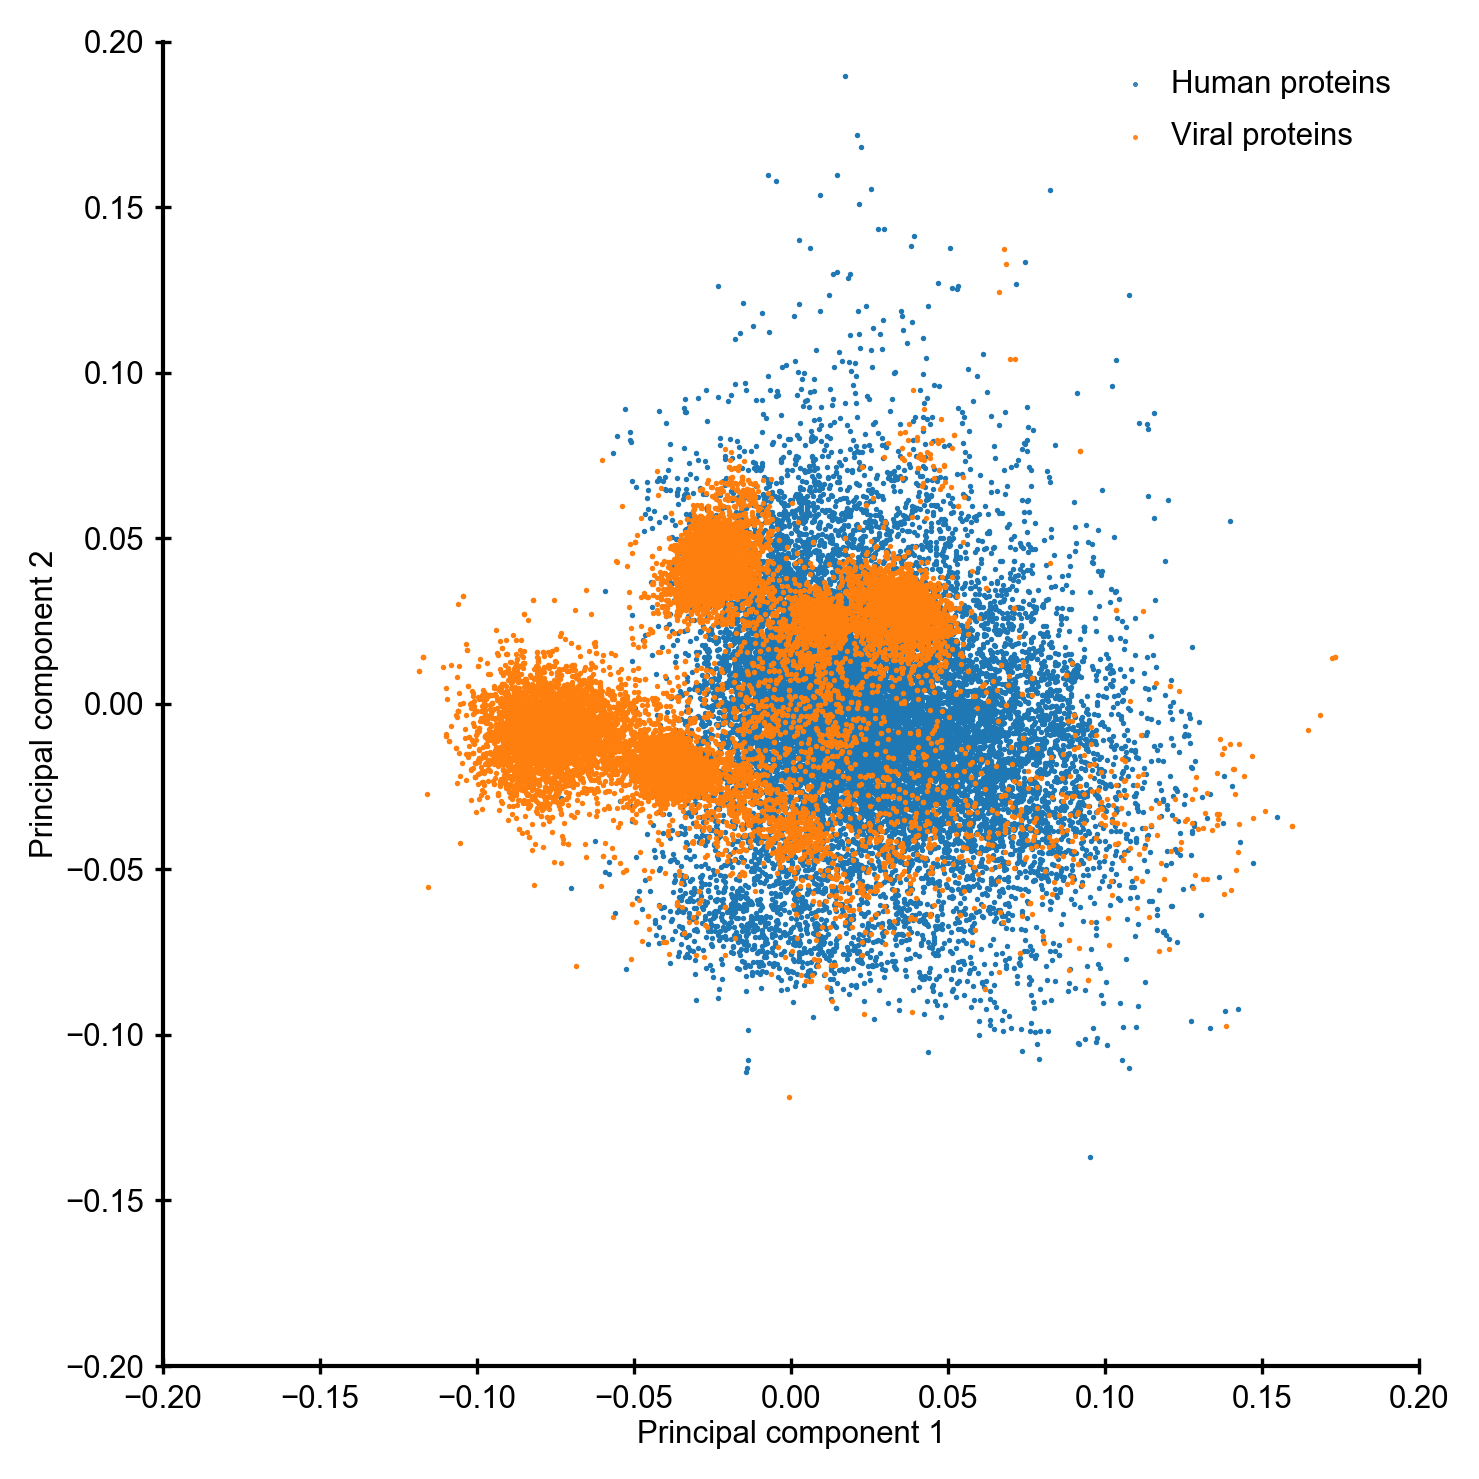
\includegraphics[width=\columnwidth]{viruses}
%    \caption{Likelihood of randomly drawn viral 9mers given a triplet model based on the human proteome statistics. B cell and T cell epitope likelihoods. Interestingly the B cell epitopes are more similar to the human proteome than if they where drawn at random.
%    \label{figviruses}
%    }
%\end{figure}


\subsection{A shell theory of immunogenicity?}

\begin{figure}
    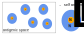
\includegraphics{shelltheorysketch}
    \caption{Sketch of the shell theory of immunogenicity: To be immunogenic an antigen needs to fall outside the tolerance region (orange), but within one of the detectable regions surrounding a self-antigen (blue).
    \label{figshelltheorysketch}
    }
\end{figure}

\begin{figure}
    \includegraphics[width=\columnwidth]{shelltheory}
    \caption{Immunogenicity as a function of the likelihood a peptide in the shell model. The probability of a peptide being immunogenic is defined as the probability of being detectable, but not tolerated. The probability of immunogenicity times the probability of peptides within the pathogen proteome (assumed to be lognormal with $mu = -1.25 k$ and $\sigma = 0.3 k$ with $k=9$) gives a hypothetical expected distribution for the epitopes, which is clipped at both ends.  
    \label{figshelltheory}
    }
\end{figure}

How likely is it that a peptide will be close enough to a self-peptide to be tolerized? How likely to be close enough such that there has been positive selection? To a first approximation neighboring peptides will have similar probabilities. Therefore the probabilities of a peptide relate to the local density and thus to the average distance to the nearest neighbor.

Consider that there is a number $N_T$ neighboring peptides that if they are in the self-peptidome would lead to tolerance, and a number $N_D > N_T$ of neighboring peptides that would lead to positive selection on TCRs recognizing the peptide and are thus needed for detectability. The probability of a peptide of probability $p$ being tolerized is $P_T \sim 1-(1-N_T p)^N$ assuming the $N$ possible self-peptides are sampled statistically independently from the peptidome distribution. As $N_T p \ll 1$ we can approximate $P_T \sim 1-e^{-N_T p N}$. Similarly, the probability of being detectable is $P_D \sim 1-(1-N_D p)^N \approx 1-e^{-N_D p N}$. Setting $N_T$ to the number of first neighbors (171 for 9mers), and $N_D$ to the number of second neighbors (25992 for 9mers) and assuming that $N$ is equal to the total possible number of kmers that can be generated from the full human proteome ($\sim 2 \cdot 10^7$), we can plot how $P_T$ and $P_D$ depends on $p$ (Fig.~\ref{figshelltheory}).

\bibliography{library}

\begin{figure}
    \includegraphics{entropyaa}
    \caption{Entropy of the single site distribution of amino acids used in different positions along proteins in the human proteome. In an overwhelming majority of cases the first amino acid in a protein is a Methionine, because this amino acid is encoded by the start codon AUG. There is a slightly lower entropy o amino acids also in the following few amino acids, which might similarly be explained by known mRNA biases around the initiation codon (rf. Kozak consensus sequence). 
    \label{figentropyaa}
    }
\end{figure}

\end{document}


